%
% file: localoperator.tex
% author: Victor Brena
% description: Briefly describes properties of the local operator.
%

\chapter{Reliability Block Diagram}
\label{app:app01}

\initial{R}eliability block diagrams, for a system as complex as a nuclear plant especially, can become huge and hard to read. In order to facilitate the reading, the case study has been divided in four systems: primary, secondary, tertiary and structure~\ref{fig:rbd_global}. For each of those systems, the redundant components are indicated by a block instead of a simple rectangle. Those blocks are then analyzed in more details in subsequent figures.

\section{Global system}

The structure is considered only for the primary circuit in the present case study. However, we could also choose to consider the secondary and tertiary circuits structure in our analyses. This would be, for example, the control room roof caving in or a plane falling on the steam generator building, etc.

\begin{figure}[!htb]
	\centering
	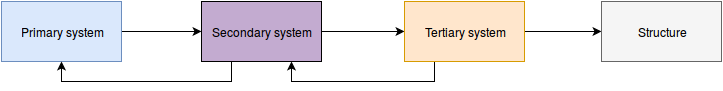
\includegraphics[height=0.1\textheight]{fig0a/main_RBD}
	\mycaption[Main Reliability Block Diagram architecture]{Main RBD architecture}
	\label{fig:rbd_global}
\end{figure}

\cleardoublepage

\section{Primary system}

\begin{figure}[!htb]
	\centering
	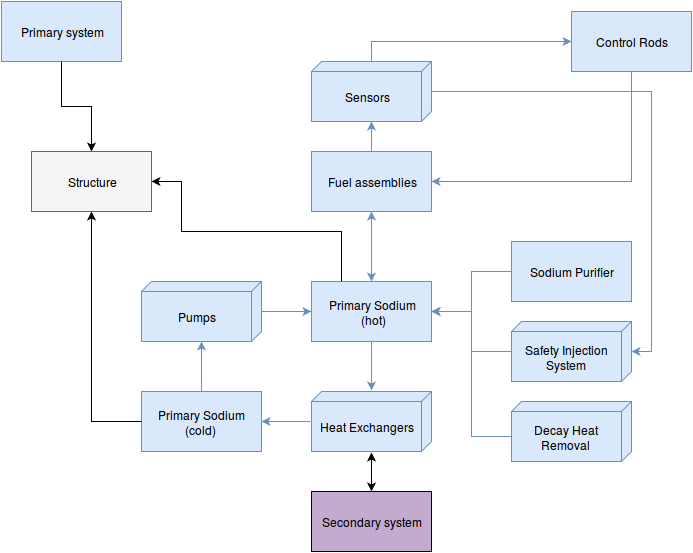
\includegraphics[height=0.6\textheight]{fig0a/Primary_system}
	\mycaption[Reliability Block Diagram for the primary system]{Reliability Block Diagram for the primary system}
	\label{fig:rbd_primary}
\end{figure}

\newpage
\subsection{Primary system redundancies}

\begin{figure}[!htb]
	\centering
	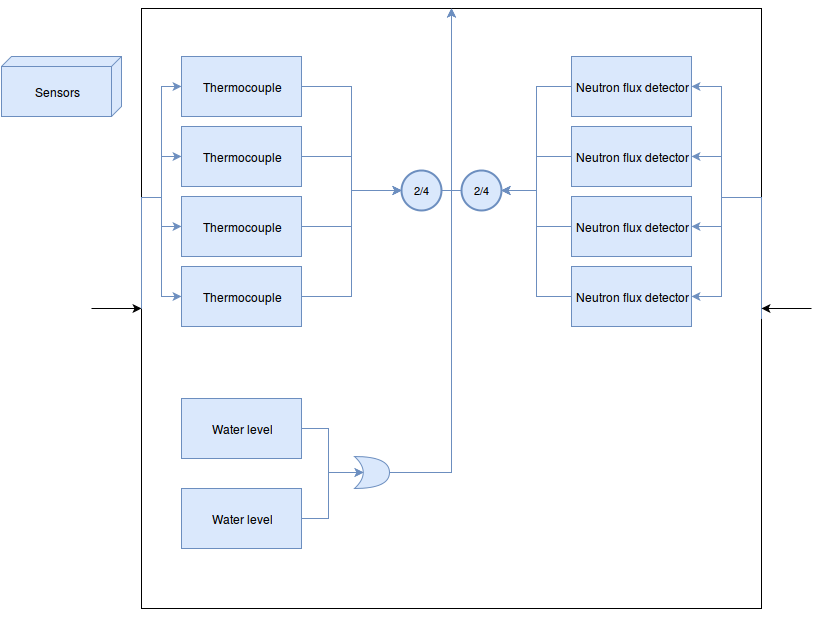
\includegraphics[height=0.55\textheight]{fig0a/primary/Primary_sensors_subsystem}
	\mycaption[Reliability Block Diagram for the core sensors in the primary system]{Reliability Block Diagram for the core sensors in the primary system}
	\label{fig:rbd_primary_sensors}
\end{figure}

\begin{figure}[!htb]
	\centering
	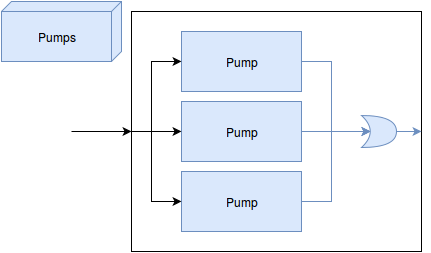
\includegraphics[height=0.4\textheight]{fig0a/primary/Primary_Pump_subsystem}
	\mycaption[Reliability Block Diagram for the primary pumps in the primary system]{Reliability Block Diagram for the primary pumps in the primary system}
	\label{fig:rbd_primary_pumps}
\end{figure}

\begin{figure}[!htb]
	\centering
	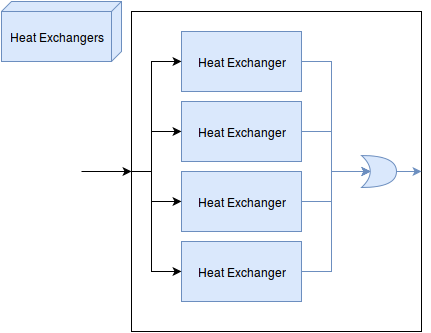
\includegraphics[height=0.5\textheight]{fig0a/primary/Primary_HX_subsystem}
	\mycaption[Reliability Block Diagram for the heat exchangers in the primary system]{Reliability Block Diagram for the heat exchangers in the primary system}
	\label{fig:rbd_primary_hx}
\end{figure}

\begin{figure}[!htb]
	\centering
	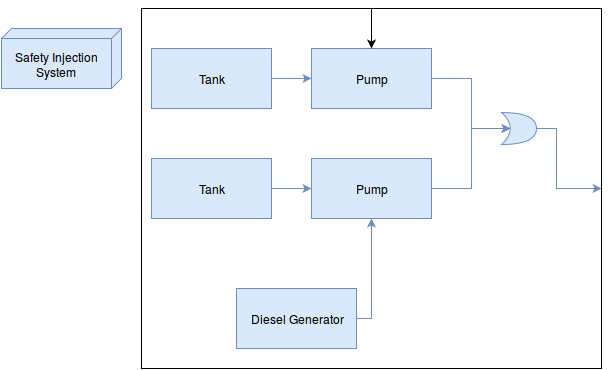
\includegraphics[height=0.45\textheight]{fig0a/primary/Primary_SIS_subsystem}
	\mycaption[Reliability Block Diagram for the safety injection system in the primary system]{Reliability Block Diagram for the safety injection system in the primary system}
	\label{fig:rbd_primary_sis}
\end{figure}

\begin{figure}[!htb]
	\centering
	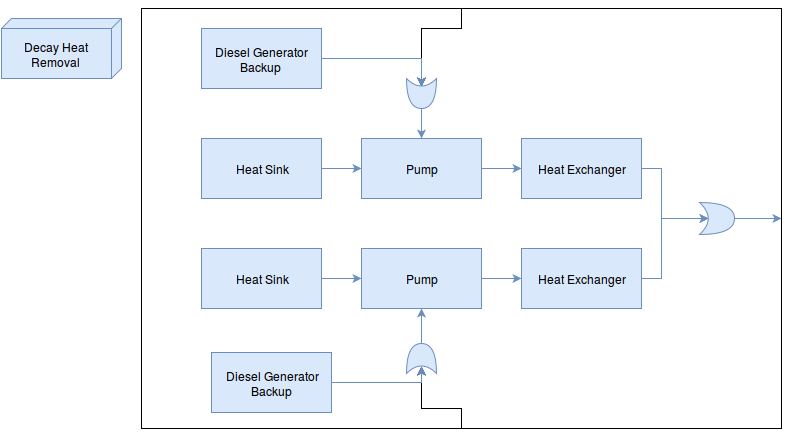
\includegraphics[height=0.4\textheight]{fig0a/primary/Primary_DHR_subsystem}
	\mycaption[Reliability Block Diagram for the decay heat removal in the primary system]{Reliability Block Diagram for the decay heat removal in the primary system}
	\label{fig:rbd_primary_dhr}
\end{figure}

\cleardoublepage

\section{Secondary system}

\begin{figure}[!htb]
	\centering
	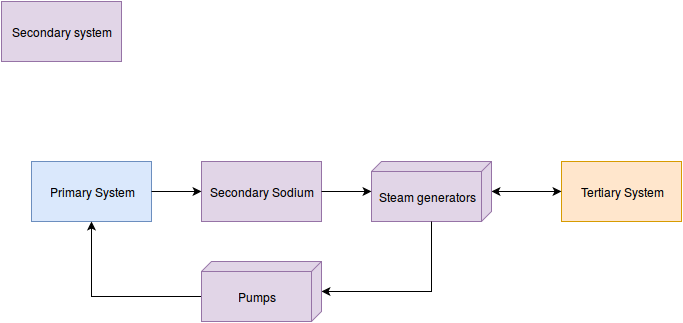
\includegraphics[height=0.35\textheight]{fig0a/Secondary_system}
	\mycaption[Reliability Block Diagram for the secondary system]{Reliability Block Diagram for the secondary system}
	\label{fig:rbd_secondary}
\end{figure}

\newpage
\subsection{Secondary system redundancies}

\begin{figure}[!htb]
	\centering
	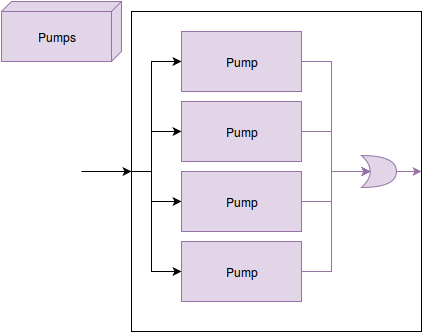
\includegraphics[height=0.5\textheight]{fig0a/secondary/Secondary_Pump_subsystem}
	\mycaption[Reliability Block Diagram for the secondary pumps in the secondary system]{Reliability Block Diagram for the secondary pumps in the secondary system}
	\label{fig:rbd_secondary_pumps}
\end{figure}

\begin{figure}[!htb]
	\centering
	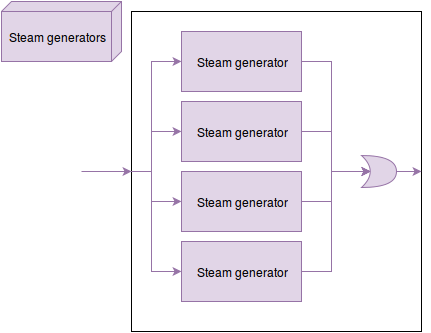
\includegraphics[height=0.5\textheight]{fig0a/secondary/Secondary_SG_subsystem}
	\mycaption[Reliability Block Diagram for the steam generators in the secondary system]{Reliability Block Diagram for the steam generators in the secondary system}
	\label{fig:rbd_secondary_sg}
\end{figure}

\cleardoublepage

\section{Tertiary system}

\begin{figure}[!htb]
	\centering
	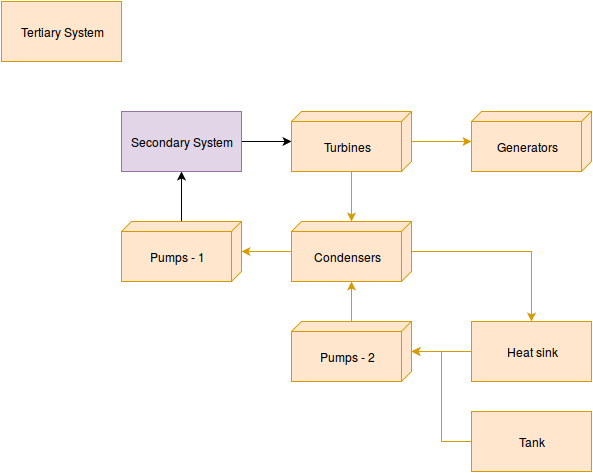
\includegraphics[height=0.5\textheight]{fig0a/Tertiary_system}
	\mycaption[Reliability Block Diagram for the tertiary system]{Reliability Block Diagram for the tertiary system}
	\label{fig:rbd_tertiary}
\end{figure}

\newpage
\subsection{Tertiary system redundancies}

\begin{figure}[!htb]
	\centering
	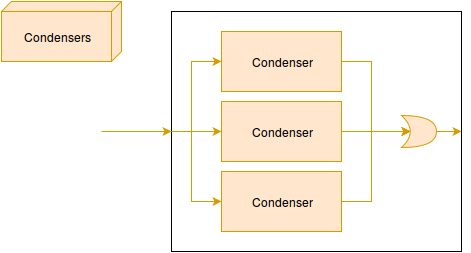
\includegraphics[height=0.35\textheight]{fig0a/tertiary/Tertiary_Subsystem_condensers}
	\mycaption[Reliability Block Diagram for the condensers in the tertiary system]{Reliability Block Diagram for the condensers in the tertiary system}
	\label{fig:rbd_tertiary_condensers}
\end{figure}

\begin{figure}[!htb]
	\centering
	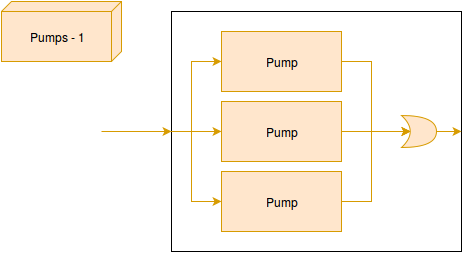
\includegraphics[height=0.35\textheight]{fig0a/tertiary/Tertiary_Subsystem_Pumps1}
	\mycaption[Reliability Block Diagram for the tertiary-secondary pumps in the tertiary system]{Reliability Block Diagram for the tertiary-secondary pumps in the tertiary system}
	\label{fig:rbd_tertiary_pumps1}
\end{figure}

\begin{figure}[!htb]
	\centering
	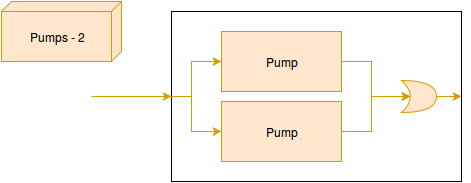
\includegraphics[height=0.25\textheight]{fig0a/tertiary/Tertiary_Subsystem_Pumps2}
	\mycaption[Reliability Block Diagram for the boundary-tertiary pumps in the tertiary system]{Reliability Block Diagram for the boundary-tertiary pumps in the tertiary system}
	\label{fig:rbd_tertiary_pumps2}
\end{figure}

\begin{figure}[!htb]
	\centering
	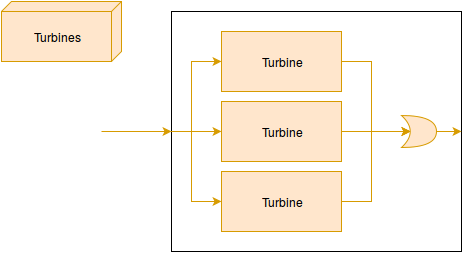
\includegraphics[height=0.35\textheight]{fig0a/tertiary/Tertiary_Subsystem_Turbines}
	\mycaption[Reliability Block Diagram for the turbines in the tertiary system]{Reliability Block Diagram for the turbines in the tertiary system}
	\label{fig:rbd_tertiary_turbines}
\end{figure}

\begin{figure}[!htb]
	\centering
	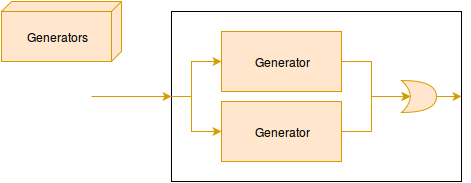
\includegraphics[height=0.25\textheight]{fig0a/tertiary/Tertiary_Subsystem_Generators}
	\mycaption[Reliability Block Diagram for the generators in the tertiary system]{Reliability Block Diagram for the generators in the tertiary system}
	\label{fig:rbd_tertiary_generators}
\end{figure}





\
